\problemname{Tower of Hanoi}

We are going to solve the \emph{Tower of Hanoi} puzzle.
The objective is to move all of the discs from the left-most pillar to the right-most pillar.
There are two simple rules:
\begin{itemize}
    \item We can only move one disc at a time.
    \item We can never place a disc on top of another disc that is smaller than the disc being moved.
\end{itemize}


\begin{figure}[h]
    \centering
    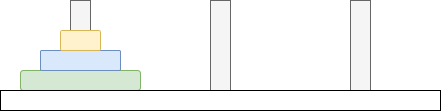
\includegraphics[width=0.5\textwidth]{tower}
    \caption{\texttt{Tower of hanoi}}
\end{figure}

The number of discs can vary.
In our examples we will assume that there are only $3$  to $5$ discs
but our solution should be able to handle up to $9$ discs.

Having unleashed the power of functions,
we can take a divide-and-conquer approach
to break the Tower of Hanoi problem into smaller problems and solve them individually.


\textbf{Note that we are testing your code differently in these following tasks,
please only submit your function definitions, without any code outside the functions!}
The main python files, which will handle input and output, are already provided.
You can download and place the main files in the same directory as your python file.
You can then run the main python files we provide to try out the samples.

